\section{Implementation}
This project was very implementation heavy and low level. It required getting a key understanding of C, how pointer-casting works in C, and virtual method tables. This section details the implementation of this project, which had two major parts: the tracing garbage collector implemented in C from scratch, and the compiler C-backend outputting C code which uses the garbage collector.

\subsection{Theoretical Background}
% If you are using theoretical concepts, explain them first in this subsection. Even if they come from the course (e.g., lattices), try to explain the essential points \emph{in your own words}. Cite any reference work you used like this \cite{TigerBook}. This should convince us that you know the theory behind what you coded.
As stated, this project was more implementation heavy and quite low level, rather than theoretical but it relies on a few established concepts that I had to research.

\subsubsection{Garbage collection strategies}
There are two major ways garbage collection is implemented. The first one, and perhaps most common, is a tracing garbage collector. In this strategy you have "GC pauses" where the garbage collector runs and tries to establish which part of the heap is currently used and which can be freed. This typically requires a runtime, like the JVM. In a tracing garbage collector the GC will scan the stack, global variables, and so on for references to GC-allocated memory. These are called the roots of the reference tree. Each reference may itself contain references to other instances, this is what forms the tree structure. While visiting each node in the tree the GC will mark these as used, and will then discard all memory that was not marked. This works because the memory that wasn't marked is fundamentally unreachable by the program and can thus safely be reclaimed. This strategy, as well as other much more sophisticated techniques is used in the JVM, and the V8 JS engine for example \cite{v8-gc}.

The other major strategy is reference counting. In this strategy each instance of an object has a count of how many references exist to the instance. Every time such a reference is created the counter is incremented and everything it goes out of scope it is decremented. When it reaches zero you know there are no more references to the instance and can thus safely free the memory. A problem with this approach you need to solve is cyclic references which will never reach zero. This strategy is used in the Swift language for example \cite{swift-arc}.

For this project I chose the first approach, a tracing garbage collector.

\subsubsection{The x86\_64-architecture}
In the introduction I argued that one benefit of a C-backend is being able to target different architectures. However, my garbage collector implementation is unfortunately x86\_64-specific.

As we know, a program in the x86\_64 architecture is logically divided into segments: the stack, heap, code, and data segments. The \texttt{punkt0} language has no pointers or pointer arithmetic, as such all pointers to class instances can be found on the stack. To find all root nodes of the reference tree when garbage collecting you therefore only have to look at the stack. This was my initial thought, however, it turned out to not be that simple. Additionally, pointers to class instances can be temporarily held in any of the CPU's general purpose register. The x86\_64 CPU has the following 12: $rax$, $rbx$, $rcx$, $rdx$, $r8$, $r9$, $r10$, $r11$, $r12$, $r13$, $r14$, $r15$. Note that the additional registers, such as $rsp$, $rip$, have specific purposes and cannot store program variables. More details on this in section 3.2.1.

\subsubsection{Virtual method tables}
When programming in a relatively high-level language like Java you do not have to think about a lot of the implementation details, but how does the JVM for example know what virtual function to call? If a function takes in a class A and you give it a class B which inherits from A the JVM will correctly invoke B's version of an overridden method, despite none of that information being visible in the function body.

In C there is no such thing as inheritance so this behavior had to be implemented. This is usually done through \textit{Virtual method tables} or vtables. On a low level, a vtable is just an array of function pointers. When you dereference a class to call a method, instead of jumping to a fixed address where the function is stored, the address is looked up in the vtable. To know which vtable to use each instance of a class has to store a pointer to it's vtable \cite{vtable}. This dynamic dispatch leads to both memory and runtime overhead.

\subsection{Implementation Details}
% Describe all non-obvious tricks you used. Tell us what you thought was hard and why. If it took you time to figure out the solution to a problem, it probably means it wasn't easy and you should definitely describe the solution in detail here. If you used what you think is a cool algorithm for some problem, tell us. Do not however spend time describing trivial things (we know what a tree traversal is, for instance).
% After reading this section, we should be convinced that you knew what you were doing when you wrote your extension, and that you put some extra consideration for the harder parts.
What follows are two sections detailing the work required to implement the two major parts of this project: a tracing garbage collector implemented in C from scratch, and the compiler C-backend outputting C code which uses the garbage collector.

\subsubsection{Garbage collector in C}
For this project I implemented a stand-alone garbage collector in C from scratch (see \texttt{./c-backend/gc.h} in my repository). It is an arena-style garbage collector. On start-up it allocates a large area of memory from malloc and via it's on allocation call hands out pointers to bits of this memory. It internally keeps track of which bytes of that memory-arena are free and which are occupied.

To keep track of which bytes are free and which are occupied the GC uses a bitmap where the n:th bit indicates whether or not the n:th \textit{byte} of the memory-arena is taken. This requires an extra eighth of the total memory area for this bookkeeping and is not the most efficient approach (see more in section 4) but it was easy to implement for this proof of concept. To allocate a chunk of memory the GC scans this bitmap for a continuous number of zero bits that can fit the number of requested bytes. This requires some carefully thought-out bitwise operations but was overall not too difficult to implement. On allocation the GC prepends a header for it's own bookkeeping. This is required to keep track of how large the allocation is for example.

The GC I implemented is a tracing garbage collector, meaning at each collection phase it looks at all the nodes in the reference tree to see which allocated instances are still reachable by the program, and thus should not be freed. In punkt0 this is relatively straight forward. The roots of the reference tree can only be found on the stack, since \texttt{punkt0} does not allow any sort of pointer arithmetic, is type safe, and does not have any global variables. To find these references the GC scans the entire stack looking for values that "look like" a GC allocated pointer. This is achieved by, at initialization, storing the address of a local variable to get the address of the top of the stack, and then scanning all values from the current stack pointer up to that address.

An obvious problem here is determining what values on the stack actually are GC-heap pointers versus regular values, like an \texttt{int}, that just happen to hold a value that looks like such a pointer. While this may not be a common occurrence, I chose to try and handle this edge case with a canary strategy. In the prepended header, the GC stores a random value, called \texttt{GC\_CANARY}. When trying to determine whether or not a value on the stack is a GC-heap pointer, we compare the canary value in the header to this static value. If they are not equal, we can be sure that this was a false-positive. This reduces the probability of false-positives when tracing by a lot at the cost of a few extra bytes per allocation. Not only would a random value on the stack have to match a pointer to the memory area, a specific value would have to exist in the memory arena at a specific offset from this value. In the worst case, if this should happen, the GC will erroneously mark a value as allocated when it should not be, which only has the consequence of temporarily leaking the bytes. In regular execution this should have a next to zero probability of occurring. You could reduce the probability even more by introduction a larger canary, at the cost of additional wasted bytes for each allocation.

An additional complexity I did not foresee was that my initial assumption, that all references can be found on the stack, does not hold when compiling with optimizations enabled, i.e with \texttt{-O2/3}! When compiling with these flags my C programs, that initially worked, started to seg fault. After a lot of debugging, even pulling in $gdb$ and stepping through the program, I realized the problem. When compiling with optimizations the compiler will, whenever it can, store a variable in a register and completely skip allocating it on the stack. This meant my tracing GC did not see the values and erroneously freed them. Fixing this problem required some inline assembly, where I read the value from all general purpose registers in the CPU and scan them for GC-heap pointers (see figure 1). This is why my GC unfortunately is not portable to other architectures, although this function could be reimplemented for another architecture.

\begin{figure}[H]
    \centering
    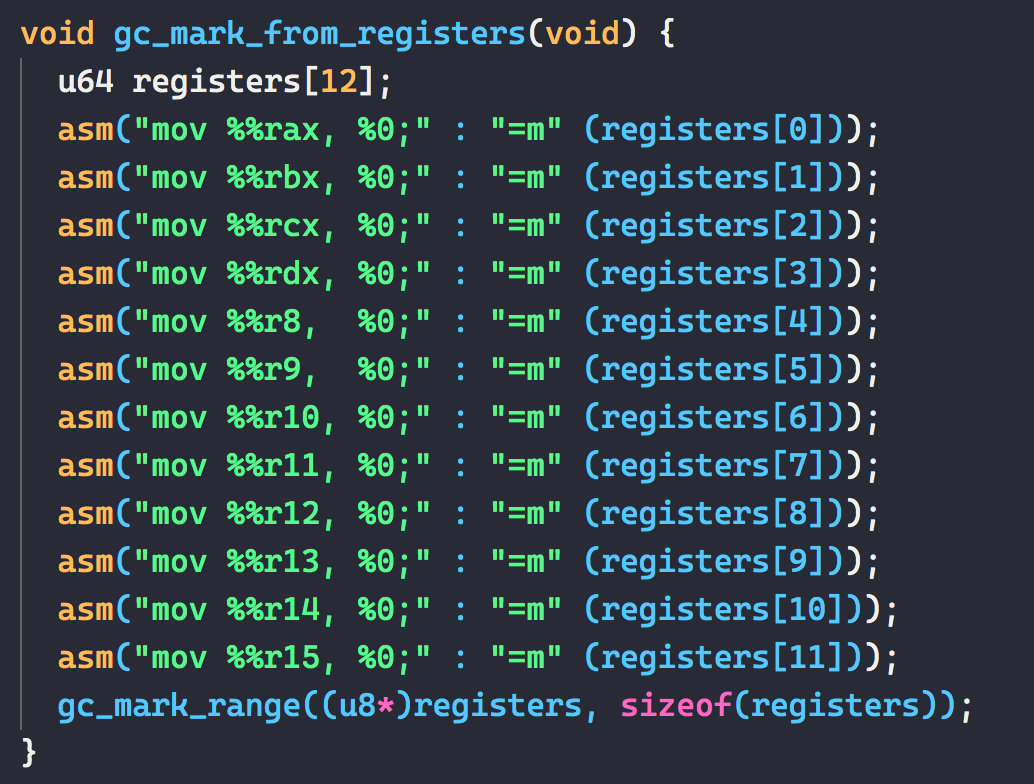
\includegraphics[width=0.40\textwidth]{imgs/gc-inline-asm.png}
    {\\ \scriptsize Figure 1: Collecting root references from the CPU registers}
\end{figure}

To summarize, in each garbage collection the GC does the following:
\begin{enumerate}
    \item Completely clear the memory bitmap, i.e mark everything in the area as \textit{free}.
    \item Using inline assembly, store all values from the 12 general purpose registers of the CPU into an array. Scan that array for root references to GC-allocated objects.
    \item Scan the entire stack for root references to GC-allocated objects.
    \item Recursively, mark all found pointers and scan the memory of the allocation for references to additional GC-allocated instances. We know how large the allocated pointer is by looking at the prepended GC header.
\end{enumerate}
The last step is very important. An instance of a \texttt{punkt0} class can have other class instances as fields, which will themselves also be GC-heap allocated. Thus they also need to be marked as allocated if their parent is still reachable. Another problem I encountered here was cyclical references. If you are not careful, the tracing algorithm will end up in an infinite loop if you blindly follow references. I handle this by checking if the memory has already been marked, before following it's references.

\subsubsection{The C code generator}
The C code generator (found in \texttt{CBackend.scala} in the repository) works a lot like the pretty-printer we implemented in lab 3. For each type of AST node it outputs a string with equivalent C code. I will not explain the implementation of that in detail here as that was largely the same as the lab. However, there were a few things that made translating \texttt{punkt0} to C a bit complicated considering the features of the languages and how the C language works. I will cover those now.

The major problem to solve was how to handle inheritance and overridden methods, which required some substantial thought and work. The most important thing that made this possible is the following line from the C standard:
\begin{quote}
    \textit{A pointer to a structure object, suitably converted, points to its initial member (or if that member is a bit-field, then to the unit in which it resides), and vice versa. There may be unnamed padding within a structure object, but not at its beginning.}
    
    \cite{c17-standard}, page 82
\end{quote}
What this says that it is always valid to cast a pointer to \textit{a struct} to a pointer to \textit{the first field of that struct}. If a class B inherits from A we can then store a \texttt{struct A} as the first field, which makes casting a B pointer to an A pointer valid, guaranteed by the official ISO language specification \cite{c17-standard}. This is used in two places in the C backend. One is for member functions, where we simply pass in the object pointer and let C automatically downcast it to a pointer of the parent class. The other time is when accessing fields of the parent class, where we first cast to the parent type, and dereference to access the field.

Another aspect of inheritance is overriding methods. To achieve this in C I implemented a virtual method table for each class. This is essentially just a static array of \texttt{void*}, where each entry is a function pointer to the overridden function. Each member function gets assigned an index in this table and before executing it we check if this entry is non-null and if so jump to the stored function pointer instead. By storing a pointer to this table only in the uppermost parent class (i.e classes without any parent) we can again utilize the part of the C standard quoted above, to safely cast any class pointer to a vtable pointer. Also, by only storing this in the root parent class we only pay the cost of one pointer per instance, in terms of memory overhead.

If- and block-expressions are something that \texttt{punkt0} has that does not trivially map to C. To support these, I relied on a very common C language extension, which both GCC and Clang has supported for many years, called \textit{statement expressions}. It turns a block in C into an expression, returning the last statement in the block \cite{gcc-stmt-exprs}. For block expressions, this maps neatly which made it quite easy to implement. If-expressions on the other hand required some additional thought. I chose to implement them by turning the statement into a block expression, adding a temporary variable, letting each arm of the if assign to this variable, and return that variable from the block. See figure 2 for an example.

\begin{figure}
    \centering
    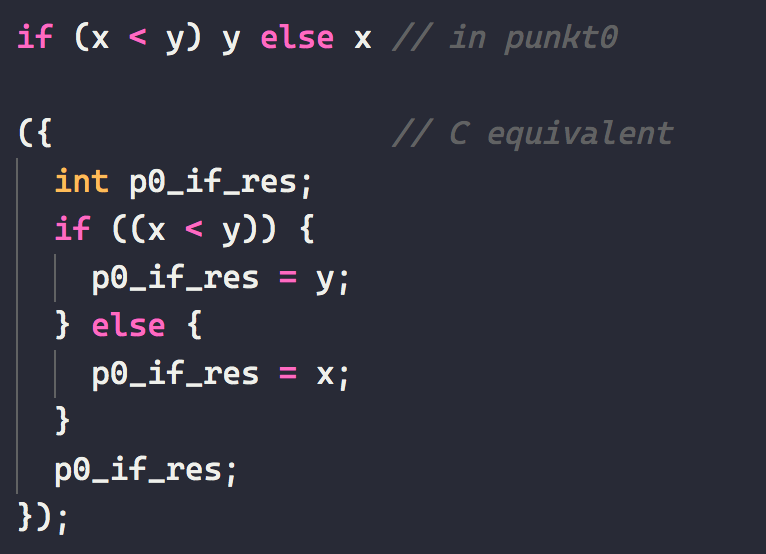
\includegraphics[width=0.45\textwidth]{imgs/if-exprs.png}
    {\\ \scriptsize Figure 2: Example of how if-expressions are transformed into C}
\end{figure}

Furthermore, identifier-clashes is also another thing I had to consider. What happens if a \texttt{punkt0} class is called \textit{garbage\_collector} when that is already defined as a struct in the GC implementation? It would not compile. To work around this I added a prefix (\texttt{p0\_}) to any identifier originating from \texttt{punkt0}, and made sure not to use that prefix in my GC implementation.

Lastly, string handling and the overloaded addition operator had to be implemented. This was done by adding three helper functions for adding strings and ints. These allocate the required memory from the garbage collector and use \texttt{sprintf} to write into that memory buffer. The C code generator then inserts a call to these functions whenever the overloaded \texttt{+} is used.